\documentclass[11pt]{article}
\usepackage[margin=1in]{geometry}
\usepackage{booktabs,graphicx,amsmath,amssymb,xcolor,float}
\usepackage{pgfplots}\pgfplotsset{compat=1.18}
\newcommand{\nstates}{2275}
\newcommand{\nq}{6825}
\newcommand{\nactions}{3}
\newcommand{\shape}{5 \times 5 \times 13 \times 7}
\newcommand{\initstate}{[0.0137, 0.0000, 3.1186, 0.0000]}
\newcommand{\inittheta}{3.1186}
\newcommand{\dt}{0.01}
\newcommand{\successsteps}{500}
\newcommand{\maxsteps}{2000}
\newcommand{\transS}{[0.0137, 0.0000, 3.1186, 0.0000]}
\newcommand{\transA}{2}
\newcommand{\transR}{-0.9997}
\newcommand{\transSn}{[0.0143, 0.1220, 3.1190, 0.0838]}
\newcommand{\outsidedeg}{178.7}
\newcommand{\epsseed}{0}
\newcommand{\epsn}{10000}
\newcommand{\nepisodes}{2000}
\newcommand{\maxepsec}{10.0}
\newcommand{\cfgalpha}{0.1}
\newcommand{\cfggamma}{0.99}
\newcommand{\epsstart}{1.0}
\newcommand{\epsend}{0.05}
\newcommand{\mawindow}{50}
\newcommand{\expseeds}{0, 1, 2}
\newcommand{\outsuccess}{success after 500 steps (terminated=True, truncated=False)}
\newcommand{\outunsafe}{unsafe after 1 steps (terminated=True, truncated=False)}
\newcommand{\outtimeout}{timeout after 50 steps (terminated=False, truncated=True)}
\title{COSC 527 Homework 2: Building and Verifying a Tabular RL Agent}
\author{Joshua Stenger}
\date{}
\begin{document}
\maketitle

\noindent\textbf{Note on supplied code.} The supplied \texttt{furuta\_env.py} was a balancing task (upright start, termination at $20^\circ$). I modified it in place for swing-up: downward start, wrapped $\widetilde\theta$, termination only on the arm limit, a five-second success criterion and an explicit \texttt{outcome} field, and the reward $\cos\widetilde\theta-0.001\tau^2$ ($-10$ on unsafe termination).

\section{Environment and episode logic}
\texttt{reset()} returned $x=\initstate$ ($[\phi,\dot\phi,\theta,\dot\theta]$): the arm is near zero and at rest, and the pendulum hangs near the downward equilibrium ($\widetilde\theta=\inittheta$\,rad, $|\widetilde\theta|\approx\pi$) at rest.
\begin{center}\begin{tabular}{cc}
\toprule
Action index & Torque [N\,m] \\
\midrule
0 & -0.02 \\
1 & +0.00 \\
2 & +0.02 \\
\bottomrule
\end{tabular}\end{center}
Sampled transition (action 2): $S_t=\transS$, $A_t=\transA$, $R_{t+1}=\transR$, $S_{t+1}=\transSn$.

\textbf{Outcomes} ($dt=\dt$\,s, success needs \successsteps{} consecutive steps in $|\widetilde\theta|\le20^\circ$, time limit \maxsteps{} steps): success: \outsuccess; unsafe (arm $|\phi|>\pi$): \outunsafe; time limit: \outtimeout. Success and unsafe are \emph{terminations}; the time limit is \emph{truncation}.

\textbf{Outside the upright region.} After one step from the start, $\widetilde\theta=\outsidedeg^\circ$ and \texttt{terminated} was false, confirming that leaving $|\widetilde\theta|\le20^\circ$ does not end an episode. Terminating there would end every episode on its first step (it starts at the bottom, $\approx180^\circ$ from upright), so the agent could never experience the swinging needed to reach the upright region.

\section{State discretization}
\begin{center}\begin{tabular}{llcp{6.5cm}}
\toprule
Variable & Selected range & Bins & Reason \\
\midrule
$\phi$ & $[-\pi,\pi]$ & 5 & Arm must stay in $\pm\pi$ (unsafe limit); coarse, since $\phi$ only matters near the limit. \\
$\dot\phi$ & $[-10,10]$ & 5 & 0.02\,N\,m gives about 11\,rad/s$^2$ near the bottom, so speeds of order 10\,rad/s occur; outer bins are open-ended. \\
$\widetilde\theta$ & $[-\pi,\pi]$ & 13 & Edges at $\pm20^\circ$ make the center bin the success region; finer near upright, one split at $\pm\pi$. \\
$\dot\theta$ & $[-8,8]$ & 7 & Natural frequency about 6.9\,rad/s; $\pm8$\,rad/s covers typical swings, outer bins catch the rest. \\
\bottomrule
\end{tabular}\end{center}
Resulting sizes: $|\mathcal S|=\shape=\nstates$ and $|Q|=|\mathcal S|\,n_a=\nstates\cdot\nactions=\nq$.
Out-of-range values are mapped by \texttt{numpy.digitize} on the \emph{internal} edges, so the first and last bins are open-ended and any value below/above the range falls in the first/last bin; $\theta$ is wrapped to $[-\pi,\pi]$ before binning, and a value exactly on an edge belongs to the upper bin. Non-finite states raise an error.
\begin{center}\small\begin{tabular}{lcc}
\toprule
Test & Continuous state & Tuple / index \\
\midrule
upright & $[0.000, 0.000, 0.000, 0.000]$ & (2, 2, 6, 3) / 1137 \\
downward (+pi) & $[0.000, 0.000, 3.142, 0.000]$ & (2, 2, 12, 3) / 1179 \\
downward (-pi) & $[0.000, 0.000, -3.142, 0.000]$ & (2, 2, 0, 3) / 1095 \\
theta near +pi & $[0.000, 0.000, 3.132, 0.000]$ & (2, 2, 12, 3) / 1179 \\
theta near -pi & $[0.000, 0.000, -3.132, 0.000]$ & (2, 2, 0, 3) / 1095 \\
theta = pi+0.01 (wraps) & $[0.000, 0.000, 3.152, 0.000]$ & (2, 2, 0, 3) / 1095 \\
theta on +20 deg boundary & $[0.000, 0.000, 0.349, 0.000]$ & (2, 2, 7, 3) / 1144 \\
theta just below boundary & $[0.000, 0.000, 0.349, 0.000]$ & (2, 2, 6, 3) / 1137 \\
phi\_dot below range & $[0.000, -100.000, 0.000, 0.000]$ & (2, 0, 6, 3) / 955 \\
phi\_dot above range & $[0.000, 100.000, 0.000, 0.000]$ & (2, 4, 6, 3) / 1319 \\
theta\_dot below range & $[0.000, 0.000, 0.000, -100.000]$ & (2, 2, 6, 0) / 1134 \\
theta\_dot above range & $[0.000, 0.000, 0.000, 100.000]$ & (2, 2, 6, 6) / 1140 \\
phi above range & $[4.000, 0.000, 0.000, 0.000]$ & (4, 2, 6, 3) / 2047 \\
\bottomrule
\end{tabular}\end{center}

\section{Epsilon-greedy verification}
Implementation: with probability $\epsilon$ sample uniformly from \emph{all} actions (greedy ones included); otherwise choose uniformly among tied greedy actions. For $Q(s^\dagger,\cdot)=[1,2,2]$ the implied probabilities are $\epsilon/3$ for action 0 and $\epsilon/3+(1-\epsilon)/2$ for actions 1 and 2. Seed \epsseed, \epsn{} samples, $Q$ unchanged:
\begin{center}\begin{tabular}{llccc}
\toprule
$\epsilon$ &  & action 0 & action 1 & action 2 \\
\midrule
0.20 & observed & 0.0663 & 0.4705 & 0.4632 \\
 & implied & 0.0667 & 0.4667 & 0.4667 \\
0.00 & observed & 0.0000 & 0.5037 & 0.4963 \\
 & implied & 0.0000 & 0.5000 & 0.5000 \\
\bottomrule
\end{tabular}\end{center}
At $\epsilon=0$ action 0 is never chosen and the two tied greedy actions split about 50/50, since exploration is off and ties are broken uniformly.

\section{SARSA and Q-learning update audit}
\begin{center}\small\begin{tabular}{lccc}
\toprule
Nonterminal &  &  &  \\
\midrule
$S_t, A_t$ & 1179, 2 &  &  \\
$R_{t+1}$ & -1.0000 &  &  \\
$S_{t+1}, A_{t+1}$ & 1095, 0 &  &  \\
$Q_{old}(S_t,A_t)$ & 0.5000 &  &  \\
$Q_{old}(S_{t+1},\cdot)$ & $[1.0000, 3.0000, 2.0000]$ &  &  \\
$\alpha,\gamma$ & 0.1, 0.9 &  &  \\
 &  & SARSA & Q-learning \\
Target $Y$ &  & -0.1000 & 1.7000 \\
$Q_{new}(S_t,A_t)$ &  & 0.4400 & 0.6200 \\
\bottomrule
\end{tabular}
\medskip
\begin{tabular}{lccc}
\toprule
Terminal &  &  &  \\
\midrule
$R_{t+1}$ (terminal) & -10.0000 &  &  \\
$Q(S_{t+1},\cdot)$ variant 1 & $[1.0000, 3.0000, 2.0000]$ &  &  \\
$Q(S_{t+1},\cdot)$ variant 2 & $[1000000.0, -1000000.0, 5.0]$ &  &  \\
 &  & SARSA & Q-learning \\
Target $Y$ (both variants) &  & -10.0000 & -10.0000 \\
$Q_{new}(S_t,A_t)$ &  & -0.5500 & -0.5500 \\
\bottomrule
\end{tabular}\end{center}
Both targets use the same stored transition. $Y^{\text{SARSA}}=R_{t+1}+\gamma Q(S_{t+1},A_{t+1})$ and $Y^{Q}=R_{t+1}+\gamma\max_a Q(S_{t+1},a)$; the program output matched the hand calculation (asserted in \texttt{audit\_updates.py}). The two targets are equal when the next action $A_{t+1}$ is a greedy action in $S_{t+1}$ (for example the greedy policy or $\epsilon=0$) and differ when exploration picks a non-greedy $A_{t+1}$. For the terminal transition the continuation value is zero, so $Y=R_{t+1}$ whatever values are stored for $S_{t+1}$ (two very different next-state rows give identical results).

\section{Preliminary learning experiment}
Q-learning; seeds \expseeds; \nepisodes{} episodes; $\alpha=\cfgalpha$, $\gamma=\cfggamma$; $\epsilon$ decays linearly from \epsstart{} to \epsend{}; $Q\equiv0$ initially; maximum episode duration \maxepsec\,s. Moving average window \mawindow. Evaluation: frozen $Q$, $\epsilon=0$, no updates, one greedy episode per seed.
\begin{center}\small\begin{tabular}{cccccrr}
\toprule
Seed & Final MA return & Final MA dur. & Visited frac. & Eval. behavior & Max dev. from down [$^\circ$] & Min $|\widetilde\theta|$ [$^\circ$] \\
\midrule
0 & -235.80 & 260 & 0.261 & growing\_swing & 47.6 & 132.4 \\
1 & -305.55 & 392 & 0.249 & growing\_swing & 55.8 & 124.2 \\
2 & -217.89 & 245 & 0.235 & growing\_swing & 61.3 & 118.7 \\
\bottomrule
\end{tabular}\end{center}
\begin{figure}[H]\centering
\begin{minipage}{.48\linewidth}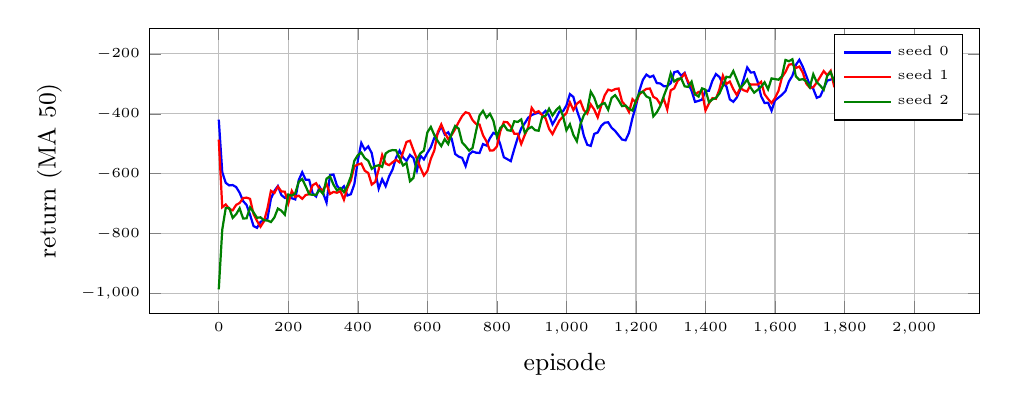
\begin{tikzpicture}
\begin{axis}[width=\linewidth,height=5.2cm,grid=major,xlabel={episode},ylabel={return (MA 50)},legend style={font=\tiny},label style={font=\small},tick label style={font=\tiny}]
\addplot[thick,color=blue] coordinates {(0,-419.2) (10,-594.7) (20,-630.4) (30,-638.9) (40,-637.8) (50,-644.4) (60,-663.4) (70,-691.2) (80,-704.2) (90,-736.9) (100,-774.6) (110,-780.6) (120,-760.5) (130,-756.6) (140,-749.8) (150,-683.3) (160,-657.3) (170,-641.2) (180,-671) (190,-680.7) (200,-680.3) (210,-681.7) (220,-685.7) (230,-621.3) (240,-595) (250,-620.2) (260,-620.4) (270,-665.7) (280,-676) (290,-643.7) (300,-664.3) (310,-696.4) (320,-604.2) (330,-602.5) (340,-639.9) (350,-652.6) (360,-641.9) (370,-672.6) (380,-668.3) (390,-634.5) (400,-556.3) (410,-497.1) (420,-520.2) (430,-508.7) (440,-531.3) (450,-592.8) (460,-649.9) (470,-618.1) (480,-641.8) (490,-608.8) (500,-585.5) (510,-546.6) (520,-523.3) (530,-545.4) (540,-557.1) (550,-537.2) (560,-547.6) (570,-589.1) (580,-539.8) (590,-551.9) (600,-530.3) (610,-511.5) (620,-480) (630,-465.6) (640,-441) (650,-469.4) (660,-461.6) (670,-483.7) (680,-534.1) (690,-542.8) (700,-547.1) (710,-574.5) (720,-535.7) (730,-525.7) (740,-529.7) (750,-530.7) (760,-501) (770,-505.8) (780,-481) (790,-463.5) (800,-469.6) (810,-503.4) (820,-544.9) (830,-551.3) (840,-557.9) (850,-517.3) (860,-479.4) (870,-448.3) (880,-431.6) (890,-413) (900,-404.1) (910,-399.4) (920,-396.3) (930,-401.5) (940,-390) (950,-405.8) (960,-435.2) (970,-415.6) (980,-392.1) (990,-391.8) (1000,-372) (1010,-334.2) (1020,-343.6) (1030,-388.2) (1040,-421.9) (1050,-473.3) (1060,-503.4) (1070,-507) (1080,-467) (1090,-462.2) (1100,-440.4) (1110,-429.7) (1120,-428.2) (1130,-446.6) (1140,-457) (1150,-471.7) (1160,-485.7) (1170,-488.4) (1180,-463.3) (1190,-413.5) (1200,-373) (1210,-322) (1220,-286.6) (1230,-269) (1240,-277.4) (1250,-272.6) (1260,-297.3) (1270,-298.7) (1280,-307.8) (1290,-307.5) (1300,-297.8) (1310,-261.1) (1320,-257.8) (1330,-272.8) (1340,-263.2) (1350,-297.2) (1360,-323.3) (1370,-360.1) (1380,-356.8) (1390,-352.8) (1400,-322.7) (1410,-322.8) (1420,-289.2) (1430,-267.2) (1440,-277.1) (1450,-299.4) (1460,-307.9) (1470,-351.8) (1480,-359.8) (1490,-345.5) (1500,-319.5) (1510,-283) (1520,-245.2) (1530,-261.8) (1540,-261.4) (1550,-293.1) (1560,-341.4) (1570,-364) (1580,-362.8) (1590,-389.6) (1600,-355.1) (1610,-345.8) (1620,-336.2) (1630,-324.1) (1640,-291.9) (1650,-272.8) (1660,-236.5) (1670,-219.5) (1680,-243.3) (1690,-273.4) (1700,-304.1) (1710,-316.8) (1720,-346.5) (1730,-341.7) (1740,-315.4) (1750,-289.2) (1760,-285.6) (1770,-282.3) (1780,-266) (1790,-285.5) (1800,-325) (1810,-339) (1820,-315.2) (1830,-312) (1840,-342.5) (1850,-340.3) (1860,-350) (1870,-368.9) (1880,-354.2) (1890,-304.1) (1900,-312.1) (1910,-307.1) (1920,-308.1) (1930,-333.6) (1940,-348.9) (1950,-362.3) (1960,-352.9) (1970,-326.6) (1980,-302.5) (1990,-283)};
\addlegendentry{seed 0}
\addplot[thick,color=red] coordinates {(0,-486.1) (10,-711.7) (20,-702.5) (30,-717.3) (40,-722.1) (50,-704) (60,-697.7) (70,-681.3) (80,-679.7) (90,-683.9) (100,-734.5) (110,-757.6) (120,-776.7) (130,-758.9) (140,-716.2) (150,-657.1) (160,-664.3) (170,-642.9) (180,-659) (190,-660) (200,-699.1) (210,-657.4) (220,-677.4) (230,-673.3) (240,-683.7) (250,-671.2) (260,-668.1) (270,-638.2) (280,-631.6) (290,-650.6) (300,-654.7) (310,-633.6) (320,-667.4) (330,-660.6) (340,-663.4) (350,-658.1) (360,-686.7) (370,-646.9) (380,-621.8) (390,-575.1) (400,-569.2) (410,-565.8) (420,-590.1) (430,-597.4) (440,-636.2) (450,-627.3) (460,-585.7) (470,-537.2) (480,-566.1) (490,-571.4) (500,-561.5) (510,-553.5) (520,-562) (530,-528.4) (540,-493.8) (550,-489.7) (560,-521.2) (570,-551) (580,-580.1) (590,-605.9) (600,-591) (610,-550.2) (620,-522.1) (630,-460.7) (640,-435.3) (650,-463.3) (660,-484.4) (670,-470.4) (680,-450.9) (690,-427.8) (700,-407.5) (710,-394.6) (720,-398.6) (730,-421) (740,-433.7) (750,-435.7) (760,-471.5) (770,-491.8) (780,-522.5) (790,-522) (800,-509) (810,-457.5) (820,-426.9) (830,-428.1) (840,-442.7) (850,-466.2) (860,-466.3) (870,-500.7) (880,-471.2) (890,-444.9) (900,-380) (910,-396.6) (920,-391.2) (930,-403.9) (940,-414.9) (950,-450.1) (960,-467.8) (970,-444.6) (980,-422.2) (990,-409.5) (1000,-397.3) (1010,-361.8) (1020,-387.3) (1030,-366.1) (1040,-357.3) (1050,-387.9) (1060,-399.3) (1070,-368.7) (1080,-385.9) (1090,-411.8) (1100,-372.9) (1110,-338.3) (1120,-319.1) (1130,-323.1) (1140,-317.5) (1150,-315.4) (1160,-358.9) (1170,-372.7) (1180,-393.8) (1190,-351.1) (1200,-362.1) (1210,-334.6) (1220,-325.1) (1230,-316.7) (1240,-315.5) (1250,-343.3) (1260,-349.9) (1270,-368.4) (1280,-350.3) (1290,-385.7) (1300,-321.5) (1310,-315) (1320,-289.7) (1330,-280.8) (1340,-265.5) (1350,-293.3) (1360,-307.1) (1370,-335.7) (1380,-327) (1390,-324.7) (1400,-388.9) (1410,-365.2) (1420,-347.6) (1430,-349.9) (1440,-318.2) (1450,-272.5) (1460,-300.3) (1470,-292.3) (1480,-317.7) (1490,-337.1) (1500,-313.8) (1510,-321.5) (1520,-325.5) (1530,-301.6) (1540,-302.2) (1550,-302.4) (1560,-293.2) (1570,-334.7) (1580,-350.1) (1590,-364.1) (1600,-347.2) (1610,-323) (1620,-278) (1630,-260.3) (1640,-235.8) (1650,-233.9) (1660,-247) (1670,-242.1) (1680,-262.8) (1690,-299.2) (1700,-312.9) (1710,-311.4) (1720,-295.2) (1730,-276.4) (1740,-257.3) (1750,-271.2) (1760,-256.4) (1770,-308.3) (1780,-308.3) (1790,-325) (1800,-357.9) (1810,-366.1) (1820,-314.1) (1830,-299.9) (1840,-263.2) (1850,-196.1) (1860,-193.5) (1870,-209.6) (1880,-238.9) (1890,-242.5) (1900,-243.8) (1910,-243.2) (1920,-233.7) (1930,-221.2) (1940,-247.8) (1950,-273.2) (1960,-282.3) (1970,-298.8) (1980,-308.1) (1990,-317.3)};
\addlegendentry{seed 1}
\addplot[thick,color=green!50!black] coordinates {(0,-986.1) (10,-786.9) (20,-714.5) (30,-714.1) (40,-747.2) (50,-735.1) (60,-715.3) (70,-749.5) (80,-748.7) (90,-712.3) (100,-728.9) (110,-747) (120,-745.5) (130,-755.5) (140,-755.9) (150,-761.2) (160,-745.9) (170,-716.1) (180,-723.3) (190,-736.7) (200,-669.4) (210,-673.5) (220,-665) (230,-626.7) (240,-617.5) (250,-641.7) (260,-668.2) (270,-670.6) (280,-669.9) (290,-654.1) (300,-667.6) (310,-616.6) (320,-608.3) (330,-636.7) (340,-655.4) (350,-648) (360,-661.3) (370,-639.7) (380,-609.2) (390,-556.5) (400,-538) (410,-529.6) (420,-548) (430,-556.6) (440,-583.5) (450,-574.8) (460,-571.5) (470,-577.1) (480,-532.3) (490,-524.1) (500,-521) (510,-521.9) (520,-547.4) (530,-572.4) (540,-564.1) (550,-624.9) (560,-613.5) (570,-551.7) (580,-531.6) (590,-522.8) (600,-461.9) (610,-443.6) (620,-470.9) (630,-491.3) (640,-507.8) (650,-484.6) (660,-500.8) (670,-466) (680,-440.5) (690,-449.3) (700,-495.7) (710,-508) (720,-522.8) (730,-513.9) (740,-458.1) (750,-405.5) (760,-389.9) (770,-412.7) (780,-399.7) (790,-423.5) (800,-476.2) (810,-446.8) (820,-436.9) (830,-454.4) (840,-456.7) (850,-424.9) (860,-427) (870,-418.7) (880,-463.1) (890,-450) (900,-443.6) (910,-454.6) (920,-456.5) (930,-410.8) (940,-406.3) (950,-382.9) (960,-405.4) (970,-388.1) (980,-376.7) (990,-406.9) (1000,-455) (1010,-434.7) (1020,-470.6) (1030,-491.7) (1040,-435.9) (1050,-405) (1060,-387.7) (1070,-326.3) (1080,-345.8) (1090,-379.6) (1100,-368.6) (1110,-364.1) (1120,-386.5) (1130,-347) (1140,-337.7) (1150,-354.9) (1160,-374.3) (1170,-372.3) (1180,-383.1) (1190,-389.1) (1200,-356.2) (1210,-330.2) (1220,-325.8) (1230,-342) (1240,-347.7) (1250,-408.4) (1260,-394.8) (1270,-373.8) (1280,-340.6) (1290,-310.7) (1300,-264.4) (1310,-292.1) (1320,-283.6) (1330,-281.3) (1340,-308.2) (1350,-310.2) (1360,-292.5) (1370,-334.7) (1380,-342.4) (1390,-315) (1400,-319.5) (1410,-361.2) (1420,-351.6) (1430,-347.1) (1440,-332.3) (1450,-306.3) (1460,-276.3) (1470,-278.2) (1480,-257.2) (1490,-285.4) (1500,-314.9) (1510,-300.7) (1520,-285.7) (1530,-312.8) (1540,-329.3) (1550,-320) (1560,-309.5) (1570,-294.7) (1580,-317.9) (1590,-281.8) (1600,-284) (1610,-286.1) (1620,-274.6) (1630,-220.2) (1640,-224.3) (1650,-217.8) (1660,-275.2) (1670,-286.5) (1680,-284.1) (1690,-291.9) (1700,-311.3) (1710,-267.9) (1720,-294.4) (1730,-305.7) (1740,-319.5) (1750,-273.7) (1760,-260.6) (1770,-291.4) (1780,-316) (1790,-284.8) (1800,-293.1) (1810,-283.9) (1820,-227.4) (1830,-235.6) (1840,-260.6) (1850,-264) (1860,-256.6) (1870,-243.3) (1880,-213.6) (1890,-229.1) (1900,-243.7) (1910,-273.2) (1920,-287.6) (1930,-283.2) (1940,-257) (1950,-265.2) (1960,-256.1) (1970,-240.6) (1980,-228.7) (1990,-236)};
\addlegendentry{seed 2}
\end{axis}
\end{tikzpicture}\end{minipage}\hfill
\begin{minipage}{.48\linewidth}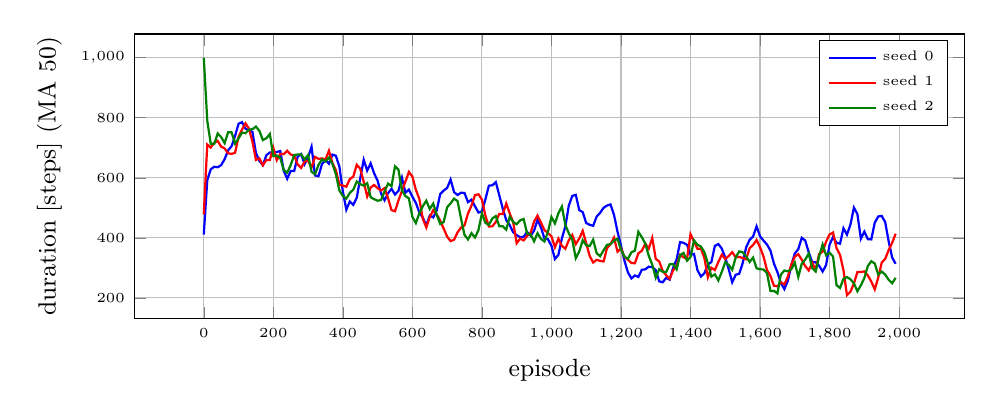
\begin{tikzpicture}
\begin{axis}[width=\linewidth,height=5.2cm,grid=major,xlabel={episode},ylabel={duration [steps] (MA 50)},legend style={font=\tiny},label style={font=\small},tick label style={font=\tiny}]
\addplot[thick,color=blue] coordinates {(0,411) (10,592) (20,628.3) (30,636.7) (40,635.1) (50,642.1) (60,662.2) (70,691.5) (80,705.3) (90,739.3) (100,779.9) (110,785.3) (120,763.4) (130,758.7) (140,752.8) (150,682.4) (160,656.2) (170,642.2) (180,675.2) (190,684.3) (200,684.2) (210,685.9) (220,689.1) (230,623.3) (240,596.7) (250,622.7) (260,622.5) (270,670.3) (280,678.9) (290,645.3) (300,668.4) (310,703.5) (320,607.7) (330,605.4) (340,645.9) (350,659.2) (360,646.9) (370,677.3) (380,673.4) (390,637.2) (400,554.7) (410,493.5) (420,521) (430,510.1) (440,533.5) (450,598.1) (460,660) (470,623.9) (480,648.1) (490,614.8) (500,590.3) (510,547.6) (520,524.9) (530,548.9) (540,563.3) (550,544.2) (560,556.6) (570,600.1) (580,550.4) (590,560.7) (600,537) (610,516.3) (620,485) (630,467.5) (640,441.6) (650,474.3) (660,468.2) (670,491.1) (680,545.7) (690,557.6) (700,566.1) (710,594.1) (720,552) (730,542.8) (740,550.4) (750,549.2) (760,518.9) (770,527.1) (780,505.4) (790,484.2) (800,488.1) (810,527.9) (820,573.7) (830,575) (840,585.5) (850,541.4) (860,497.4) (870,459.1) (880,442.2) (890,418.4) (900,409.2) (910,402) (920,403.6) (930,419.4) (940,406.9) (950,423.8) (960,459.8) (970,433.9) (980,397.3) (990,395.2) (1000,373.5) (1010,329.4) (1020,343.1) (1030,398.1) (1040,437.6) (1050,507.8) (1060,539.5) (1070,543.2) (1080,492.3) (1090,485.7) (1100,449.1) (1110,443.5) (1120,440.2) (1130,470.7) (1140,483.3) (1150,500.1) (1160,507.5) (1170,511.3) (1180,476.2) (1190,420.7) (1200,374.1) (1210,323.6) (1220,284.7) (1230,264.8) (1240,274.5) (1250,269.8) (1260,293.6) (1270,295) (1280,304) (1290,302.4) (1300,292.3) (1310,255) (1320,251.9) (1330,266.7) (1340,260.4) (1350,300) (1360,328.2) (1370,385.6) (1380,383.4) (1390,376.7) (1400,343.1) (1410,346.3) (1420,292.3) (1430,270.9) (1440,282.2) (1450,311.3) (1460,319) (1470,373) (1480,379.3) (1490,364.1) (1500,333.7) (1510,294.8) (1520,251.8) (1530,277) (1540,280) (1550,315.3) (1560,368.1) (1570,393.2) (1580,404.4) (1590,438.2) (1600,405.4) (1610,390.6) (1620,377.5) (1630,357.4) (1640,314.3) (1650,285.6) (1660,249) (1670,229.2) (1680,256.8) (1690,308.4) (1700,348) (1710,362.1) (1720,400) (1730,391.2) (1740,351.9) (1750,318.9) (1760,318.8) (1770,306.9) (1780,287.7) (1790,309.3) (1800,377.2) (1810,402.6) (1820,383.2) (1830,380.3) (1840,431.8) (1850,410.5) (1860,443.9) (1870,500.6) (1880,479.2) (1890,397.5) (1900,420.8) (1910,395.5) (1920,394.7) (1930,450.5) (1940,471.2) (1950,473) (1960,452) (1970,388.2) (1980,334.2) (1990,313.6)};
\addlegendentry{seed 0}
\addplot[thick,color=red] coordinates {(0,478) (10,710.5) (20,700.7) (30,716.6) (40,722.9) (50,703.8) (60,697.8) (70,681.6) (80,679.7) (90,683.3) (100,736.1) (110,760.8) (120,781.4) (130,763.6) (140,720.3) (150,659.5) (160,664.6) (170,641.6) (180,659) (190,659.4) (200,700) (210,658.9) (220,679.6) (230,678.7) (240,689.9) (250,677.3) (260,675) (270,644.4) (280,632.9) (290,654.1) (300,656.9) (310,634.6) (320,669.5) (330,663.1) (340,664.7) (350,660.8) (360,690.3) (370,649.4) (380,625.1) (390,577.2) (400,574.2) (410,570.3) (420,595.6) (430,603.7) (440,643.5) (450,630.3) (460,586.8) (470,537.8) (480,567.6) (490,576.1) (500,565.4) (510,557.6) (520,565.6) (530,531.8) (540,492.3) (550,488.6) (560,524.7) (570,556.3) (580,587.2) (590,619.5) (600,604.3) (610,560) (620,529.6) (630,463.6) (640,434.6) (650,469.3) (660,492.2) (670,477.9) (680,457.3) (690,431) (700,404) (710,389) (720,393.7) (730,418.3) (740,434.1) (750,441.5) (760,481.2) (770,507.1) (780,542.1) (790,545.2) (800,527.5) (810,474) (820,437.8) (830,438.2) (840,452.7) (850,479.8) (860,479.1) (870,514.3) (880,481.4) (890,451.4) (900,382) (910,397.5) (920,391.3) (930,406.8) (940,416.1) (950,453.9) (960,474.1) (970,450.5) (980,425.7) (990,415.7) (1000,405.4) (1010,368.5) (1020,397) (1030,373.2) (1040,363.6) (1050,392.1) (1060,409.6) (1070,379) (1080,397.7) (1090,423.2) (1100,382.1) (1110,339.3) (1120,317.6) (1130,326.6) (1140,323.2) (1150,321.2) (1160,366.2) (1170,379) (1180,400.6) (1190,353.8) (1200,364.6) (1210,336.1) (1220,327.1) (1230,316.4) (1240,315.1) (1250,348.3) (1260,356.9) (1270,380.4) (1280,364.1) (1290,399.6) (1300,330.1) (1310,321.1) (1320,289.9) (1330,275.4) (1340,263.3) (1350,291.7) (1360,307.3) (1370,343.4) (1380,335.1) (1390,329.6) (1400,412.4) (1410,387.7) (1420,363.1) (1430,364.4) (1440,331.9) (1450,268.8) (1460,300.3) (1470,292.7) (1480,319.3) (1490,343.7) (1500,329.1) (1510,339.6) (1520,352.1) (1530,335.1) (1540,336.4) (1550,332.8) (1560,328.6) (1570,365.3) (1580,376.2) (1590,392.6) (1600,368.9) (1610,337.6) (1620,292.4) (1630,272.7) (1640,240.2) (1650,238.3) (1660,251.7) (1670,244.8) (1680,270.8) (1690,311.2) (1700,337.5) (1710,345.4) (1720,327) (1730,305.7) (1740,291.4) (1750,316.8) (1760,293.8) (1770,345.9) (1780,353.8) (1790,387.3) (1800,411.3) (1810,417.5) (1820,365.6) (1830,343.6) (1840,291.5) (1850,209) (1860,220.5) (1870,247.7) (1880,286.3) (1890,285.7) (1900,288) (1910,274.9) (1920,254.2) (1930,228.2) (1940,267.6) (1950,317.5) (1960,330) (1970,359.1) (1980,383.1) (1990,413.8)};
\addlegendentry{seed 1}
\addplot[thick,color=green!50!black] coordinates {(0,1000) (10,790.4) (20,713.1) (30,713) (40,747.6) (50,735.6) (60,715.5) (70,752) (80,751.4) (90,713.7) (100,731.4) (110,750.6) (120,748.6) (130,760.6) (140,761.8) (150,770.7) (160,756) (170,725.7) (180,731.8) (190,745.9) (200,672.3) (210,674.2) (220,666.1) (230,625.9) (240,617) (250,642.4) (260,675.9) (270,677.4) (280,678.1) (290,661.4) (300,675.7) (310,619.8) (320,611.8) (330,642.9) (340,661.4) (350,654.5) (360,667.8) (370,646.1) (380,611.5) (390,558) (400,539.3) (410,530.5) (420,549.8) (430,560.4) (440,587.4) (450,578.9) (460,574) (470,582) (480,535.4) (490,528.7) (500,523.6) (510,525.9) (520,554.7) (530,580.7) (540,572.2) (550,638.2) (560,627) (570,557.6) (580,539.1) (590,531.4) (600,469.6) (610,449) (620,482) (630,505.2) (640,523.7) (650,496.2) (660,514.2) (670,476.8) (680,446.2) (690,452.3) (700,501.8) (710,515.1) (720,530.6) (730,522.2) (740,463.9) (750,409.5) (760,394.6) (770,415.6) (780,401.1) (790,425.2) (800,481.4) (810,449.9) (820,443) (830,464.6) (840,472.6) (850,438.2) (860,438.5) (870,427.1) (880,470.3) (890,452.6) (900,445.2) (910,458.4) (920,462.9) (930,414) (940,411.6) (950,388.2) (960,415.4) (970,396.3) (980,387.7) (990,420.1) (1000,469.5) (1010,447.8) (1020,481.8) (1030,504.3) (1040,442.8) (1050,415.1) (1060,393) (1070,332) (1080,354.4) (1090,391.9) (1100,375.2) (1110,372.6) (1120,393.7) (1130,348.8) (1140,338.7) (1150,358.4) (1160,376.6) (1170,379.2) (1180,390.8) (1190,396.8) (1200,360.4) (1210,337.5) (1220,329.9) (1230,351.6) (1240,357.1) (1250,420) (1260,402.1) (1270,380.6) (1280,339.7) (1290,310.5) (1300,267.3) (1310,295.6) (1320,286.6) (1330,285.9) (1340,311.7) (1350,312.5) (1360,294.9) (1370,342.2) (1380,349.5) (1390,323.9) (1400,335.6) (1410,391.6) (1420,376.8) (1430,370.8) (1440,351.9) (1450,315) (1460,270.6) (1470,278.5) (1480,258.1) (1490,286.6) (1500,319) (1510,309.6) (1520,293.6) (1530,334.5) (1540,354.7) (1550,351.9) (1560,338.5) (1570,319.6) (1580,334.2) (1590,298.5) (1600,295.1) (1610,294.7) (1620,282.2) (1630,222.6) (1640,223.3) (1650,214.9) (1660,277.9) (1670,291) (1680,288.5) (1690,295.2) (1700,317) (1710,269.6) (1720,313.8) (1730,327.5) (1740,347.8) (1750,298.9) (1760,288) (1770,338.3) (1780,377.9) (1790,341.7) (1800,350.6) (1810,337.6) (1820,242.5) (1830,232.9) (1840,263.5) (1850,269.3) (1860,261.9) (1870,248.3) (1880,222.1) (1890,241.5) (1900,266) (1910,305.9) (1920,322) (1930,314.2) (1940,277.5) (1950,287.6) (1960,277.2) (1970,260.1) (1980,248.4) (1990,266.6)};
\addlegendentry{seed 2}
\end{axis}
\end{tikzpicture}\end{minipage}\\[1ex]
\begin{minipage}{.48\linewidth}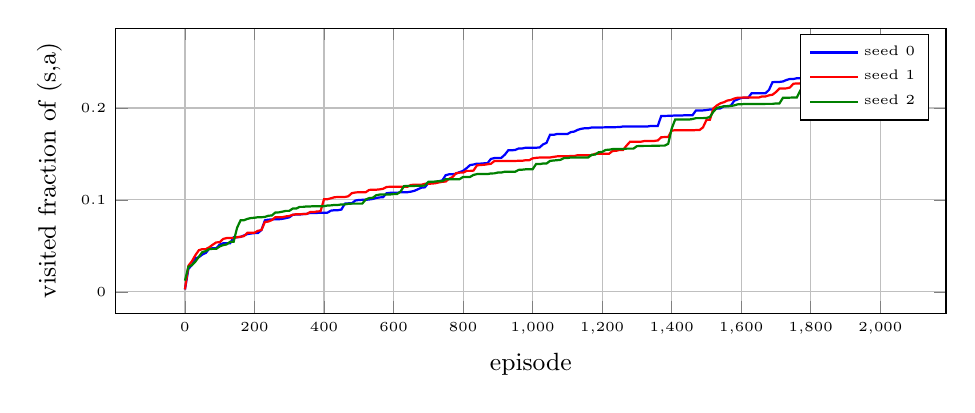
\begin{tikzpicture}
\begin{axis}[width=\linewidth,height=5.2cm,grid=major,xlabel={episode},ylabel={visited fraction of (s,a)},legend style={font=\tiny},label style={font=\small},tick label style={font=\tiny}]
\addplot[thick,color=blue] coordinates {(0,0.002637) (10,0.02491) (20,0.02916) (30,0.03648) (40,0.03766) (50,0.04059) (60,0.04234) (70,0.04689) (80,0.04747) (90,0.04747) (100,0.05143) (110,0.05275) (120,0.05275) (130,0.05289) (140,0.05934) (150,0.05934) (160,0.05978) (170,0.06139) (180,0.06286) (190,0.06344) (200,0.06388) (210,0.06403) (220,0.06725) (230,0.0778) (240,0.07853) (250,0.07868) (260,0.07897) (270,0.07897) (280,0.07941) (290,0.08015) (300,0.08103) (310,0.08381) (320,0.0841) (330,0.0841) (340,0.08454) (350,0.08484) (360,0.08586) (370,0.08586) (380,0.08586) (390,0.08601) (400,0.08601) (410,0.08615) (420,0.08835) (430,0.08879) (440,0.08879) (450,0.08952) (460,0.09597) (470,0.09626) (480,0.09626) (490,0.09934) (500,0.09993) (510,0.1001) (520,0.1001) (530,0.1005) (540,0.101) (550,0.1021) (560,0.1027) (570,0.103) (580,0.1073) (590,0.1077) (600,0.1077) (610,0.1077) (620,0.1084) (630,0.1084) (640,0.1084) (650,0.109) (660,0.1099) (670,0.1116) (680,0.1133) (690,0.1137) (700,0.1182) (710,0.1193) (720,0.1193) (730,0.1204) (740,0.1212) (750,0.1269) (760,0.1279) (770,0.1279) (780,0.1286) (790,0.1303) (800,0.1316) (810,0.1345) (820,0.1379) (830,0.1385) (840,0.1395) (850,0.1395) (860,0.1398) (870,0.1398) (880,0.1446) (890,0.1455) (900,0.1455) (910,0.1458) (920,0.1492) (930,0.154) (940,0.154) (950,0.1544) (960,0.156) (970,0.156) (980,0.1568) (990,0.1568) (1000,0.1568) (1010,0.1568) (1020,0.1571) (1030,0.1604) (1040,0.1621) (1050,0.1708) (1060,0.1708) (1070,0.1717) (1080,0.1717) (1090,0.1717) (1100,0.1717) (1110,0.1738) (1120,0.1744) (1130,0.1763) (1140,0.1774) (1150,0.178) (1160,0.178) (1170,0.1788) (1180,0.1789) (1190,0.1789) (1200,0.1789) (1210,0.179) (1220,0.179) (1230,0.179) (1240,0.1792) (1250,0.1793) (1260,0.1799) (1270,0.1799) (1280,0.1799) (1290,0.1799) (1300,0.1799) (1310,0.1799) (1320,0.1799) (1330,0.1799) (1340,0.1805) (1350,0.1805) (1360,0.1805) (1370,0.1914) (1380,0.1914) (1390,0.1915) (1400,0.1916) (1410,0.1919) (1420,0.1919) (1430,0.1919) (1440,0.1922) (1450,0.1922) (1460,0.1922) (1470,0.1974) (1480,0.1974) (1490,0.1974) (1500,0.1978) (1510,0.1984) (1520,0.1984) (1530,0.1993) (1540,0.1996) (1550,0.2019) (1560,0.2021) (1570,0.2025) (1580,0.2079) (1590,0.2094) (1600,0.211) (1610,0.2111) (1620,0.2111) (1630,0.2161) (1640,0.2161) (1650,0.2161) (1660,0.2161) (1670,0.2161) (1680,0.2198) (1690,0.2281) (1700,0.2284) (1710,0.2284) (1720,0.2289) (1730,0.2305) (1740,0.2316) (1750,0.2316) (1760,0.2324) (1770,0.2324) (1780,0.2333) (1790,0.2355) (1800,0.2372) (1810,0.2432) (1820,0.2432) (1830,0.2435) (1840,0.246) (1850,0.2467) (1860,0.2498) (1870,0.253) (1880,0.2555) (1890,0.2555) (1900,0.2579) (1910,0.2579) (1920,0.259) (1930,0.2605) (1940,0.2607) (1950,0.2607) (1960,0.261) (1970,0.261) (1980,0.261) (1990,0.261)};
\addlegendentry{seed 0}
\addplot[thick,color=red] coordinates {(0,0.002637) (10,0.02842) (20,0.03326) (30,0.03985) (40,0.04527) (50,0.04645) (60,0.04645) (70,0.0485) (80,0.05128) (90,0.05377) (100,0.05392) (110,0.05758) (120,0.05846) (130,0.05846) (140,0.05846) (150,0.05949) (160,0.05993) (170,0.06066) (180,0.06432) (190,0.06432) (200,0.06432) (210,0.06637) (220,0.06725) (230,0.07604) (240,0.07648) (250,0.0781) (260,0.08117) (270,0.08117) (280,0.08117) (290,0.08205) (300,0.08249) (310,0.08381) (320,0.0844) (330,0.0844) (340,0.08469) (350,0.08469) (360,0.08674) (370,0.08674) (380,0.08747) (390,0.08762) (400,0.1008) (410,0.1008) (420,0.1018) (430,0.1029) (440,0.1032) (450,0.1032) (460,0.1032) (470,0.104) (480,0.1073) (490,0.1081) (500,0.1084) (510,0.1084) (520,0.1084) (530,0.1109) (540,0.1111) (550,0.1111) (560,0.1115) (570,0.1121) (580,0.1141) (590,0.1143) (600,0.1143) (610,0.1143) (620,0.1143) (630,0.1143) (640,0.1143) (650,0.1163) (660,0.1165) (670,0.1165) (680,0.1165) (690,0.1175) (700,0.1175) (710,0.1178) (720,0.1181) (730,0.119) (740,0.1197) (750,0.12) (760,0.1231) (770,0.125) (780,0.1291) (790,0.1297) (800,0.1297) (810,0.1316) (820,0.1316) (830,0.1319) (840,0.1376) (850,0.138) (860,0.1382) (870,0.1388) (880,0.1393) (890,0.1423) (900,0.1423) (910,0.1423) (920,0.1423) (930,0.1424) (940,0.1424) (950,0.1424) (960,0.1426) (970,0.1426) (980,0.1432) (990,0.1432) (1000,0.1452) (1010,0.1458) (1020,0.1461) (1030,0.1461) (1040,0.1461) (1050,0.1462) (1060,0.1468) (1070,0.1474) (1080,0.1475) (1090,0.1475) (1100,0.1475) (1110,0.1478) (1120,0.1478) (1130,0.1487) (1140,0.1487) (1150,0.1487) (1160,0.1487) (1170,0.1487) (1180,0.1502) (1190,0.1503) (1200,0.1503) (1210,0.1503) (1220,0.1503) (1230,0.1533) (1240,0.1534) (1250,0.1544) (1260,0.1544) (1270,0.159) (1280,0.1632) (1290,0.1632) (1300,0.1632) (1310,0.1632) (1320,0.164) (1330,0.1642) (1340,0.1642) (1350,0.1642) (1360,0.1647) (1370,0.1682) (1380,0.1684) (1390,0.1684) (1400,0.1755) (1410,0.1758) (1420,0.1758) (1430,0.1758) (1440,0.1758) (1450,0.1758) (1460,0.1758) (1470,0.176) (1480,0.176) (1490,0.1789) (1500,0.187) (1510,0.1873) (1520,0.1996) (1530,0.2028) (1540,0.2051) (1550,0.2063) (1560,0.2081) (1570,0.2088) (1580,0.2103) (1590,0.2113) (1600,0.2113) (1610,0.2114) (1620,0.2114) (1630,0.2114) (1640,0.2114) (1650,0.2114) (1660,0.2126) (1670,0.2126) (1680,0.2138) (1690,0.2145) (1700,0.2174) (1710,0.2212) (1720,0.2212) (1730,0.2214) (1740,0.2223) (1750,0.2264) (1760,0.2268) (1770,0.2268) (1780,0.2299) (1790,0.233) (1800,0.2337) (1810,0.234) (1820,0.2346) (1830,0.2349) (1840,0.2358) (1850,0.2358) (1860,0.239) (1870,0.2394) (1880,0.2425) (1890,0.2432) (1900,0.2432) (1910,0.2432) (1920,0.2432) (1930,0.2432) (1940,0.2432) (1950,0.244) (1960,0.244) (1970,0.2448) (1980,0.2454) (1990,0.2491)};
\addlegendentry{seed 1}
\addplot[thick,color=green!50!black] coordinates {(0,0.01216) (10,0.0274) (20,0.02901) (30,0.03282) (40,0.0381) (50,0.04322) (60,0.04425) (70,0.04659) (80,0.04674) (90,0.04674) (100,0.04938) (110,0.05084) (120,0.05158) (130,0.05451) (140,0.05451) (150,0.06974) (160,0.0778) (170,0.07795) (180,0.07941) (190,0.08029) (200,0.08059) (210,0.08117) (220,0.08117) (230,0.08147) (240,0.08278) (250,0.08308) (260,0.0863) (270,0.08645) (280,0.08718) (290,0.08806) (300,0.08806) (310,0.09055) (320,0.09055) (330,0.09245) (340,0.09245) (350,0.09289) (360,0.09289) (370,0.09319) (380,0.09319) (390,0.09319) (400,0.09319) (410,0.09392) (420,0.09407) (430,0.09451) (440,0.09451) (450,0.09509) (460,0.09509) (470,0.09582) (480,0.09597) (490,0.09597) (500,0.09597) (510,0.09597) (520,0.1004) (530,0.102) (540,0.1023) (550,0.1051) (560,0.1058) (570,0.1059) (580,0.1059) (590,0.1059) (600,0.1064) (610,0.1064) (620,0.109) (630,0.115) (640,0.1152) (650,0.1152) (660,0.1152) (670,0.1155) (680,0.1155) (690,0.1156) (700,0.1197) (710,0.1197) (720,0.12) (730,0.1204) (740,0.1204) (750,0.1225) (760,0.1226) (770,0.1226) (780,0.1226) (790,0.1226) (800,0.125) (810,0.125) (820,0.125) (830,0.1272) (840,0.1281) (850,0.1281) (860,0.1281) (870,0.1281) (880,0.1288) (890,0.1289) (900,0.1298) (910,0.1298) (920,0.1307) (930,0.1307) (940,0.1307) (950,0.1307) (960,0.1327) (970,0.1329) (980,0.1333) (990,0.1333) (1000,0.1333) (1010,0.139) (1020,0.139) (1030,0.1396) (1040,0.1396) (1050,0.1424) (1060,0.1429) (1070,0.1432) (1080,0.1436) (1090,0.1455) (1100,0.1455) (1110,0.1462) (1120,0.1462) (1130,0.1462) (1140,0.1462) (1150,0.1462) (1160,0.1462) (1170,0.1492) (1180,0.1493) (1190,0.1519) (1200,0.1522) (1210,0.1544) (1220,0.1546) (1230,0.1553) (1240,0.1553) (1250,0.1553) (1260,0.1553) (1270,0.1558) (1280,0.1558) (1290,0.1558) (1300,0.1585) (1310,0.1587) (1320,0.1588) (1330,0.1588) (1340,0.1588) (1350,0.159) (1360,0.159) (1370,0.1591) (1380,0.1591) (1390,0.161) (1400,0.1776) (1410,0.1874) (1420,0.1874) (1430,0.1875) (1440,0.1875) (1450,0.1875) (1460,0.188) (1470,0.189) (1480,0.189) (1490,0.189) (1500,0.1892) (1510,0.1903) (1520,0.196) (1530,0.2001) (1540,0.201) (1550,0.2018) (1560,0.2019) (1570,0.2022) (1580,0.2029) (1590,0.204) (1600,0.2041) (1610,0.2044) (1620,0.2044) (1630,0.2044) (1640,0.2044) (1650,0.2044) (1660,0.2044) (1670,0.2045) (1680,0.2045) (1690,0.2045) (1700,0.205) (1710,0.205) (1720,0.2111) (1730,0.2111) (1740,0.2113) (1750,0.2114) (1760,0.2114) (1770,0.2192) (1780,0.222) (1790,0.222) (1800,0.222) (1810,0.2226) (1820,0.2226) (1830,0.2226) (1840,0.223) (1850,0.223) (1860,0.223) (1870,0.2233) (1880,0.2233) (1890,0.2259) (1900,0.2281) (1910,0.229) (1920,0.229) (1930,0.229) (1940,0.229) (1950,0.2303) (1960,0.2308) (1970,0.2308) (1980,0.2309) (1990,0.2315)};
\addlegendentry{seed 2}
\end{axis}
\end{tikzpicture}\end{minipage}\hfill
\begin{minipage}{.48\linewidth}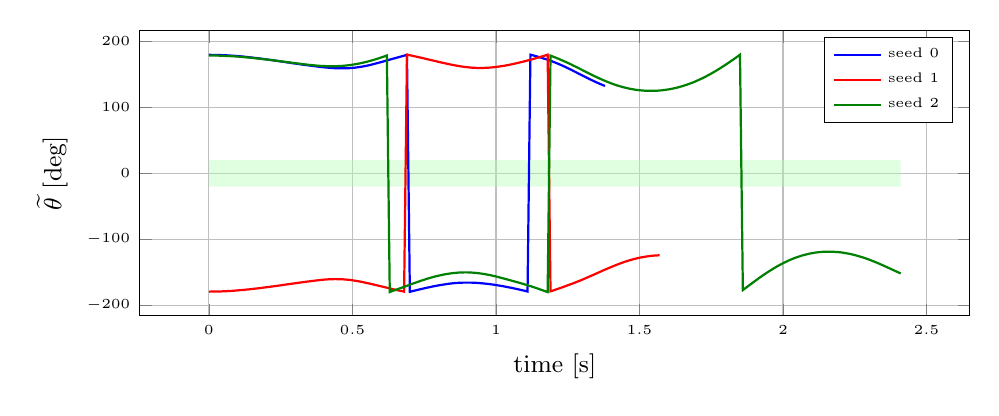
\begin{tikzpicture}
\begin{axis}[width=\linewidth,height=5.2cm,grid=major,xlabel={time [s]},ylabel={$\widetilde{\theta}$ [deg]},legend style={font=\tiny},label style={font=\small},tick label style={font=\tiny}]
\addplot[draw=none,fill=green!30,opacity=0.4,forget plot] coordinates {(0,-20) (2.41,-20) (2.41,20) (0,20)} \closedcycle;
\addplot[thick,color=blue] coordinates {(0,179.6) (0.01,179.5) (0.02,179.5) (0.03,179.4) (0.04,179.2) (0.05,179.1) (0.06,178.9) (0.07,178.6) (0.08,178.3) (0.09,178) (0.1,177.7) (0.11,177.3) (0.12,176.9) (0.13,176.4) (0.14,175.9) (0.15,175.5) (0.16,174.9) (0.17,174.4) (0.18,173.9) (0.19,173.3) (0.2,172.7) (0.21,172.1) (0.22,171.5) (0.23,170.9) (0.24,170.2) (0.25,169.6) (0.26,169) (0.27,168.3) (0.28,167.7) (0.29,167) (0.3,166.4) (0.31,165.8) (0.32,165.2) (0.33,164.5) (0.34,164) (0.35,163.4) (0.36,162.8) (0.37,162.3) (0.38,161.7) (0.39,161.2) (0.4,160.7) (0.41,160.3) (0.42,159.9) (0.43,159.6) (0.44,159.3) (0.45,159.2) (0.46,159.1) (0.47,159.1) (0.48,159.2) (0.49,159.4) (0.5,159.8) (0.51,160.2) (0.52,160.8) (0.53,161.4) (0.54,162.2) (0.55,163.1) (0.56,164) (0.57,165.1) (0.58,166.3) (0.59,167.4) (0.6,168.6) (0.61,169.8) (0.62,171.1) (0.63,172.3) (0.64,173.5) (0.65,174.7) (0.66,175.9) (0.67,177.1) (0.68,178.3) (0.69,179.4) (0.7,-179.5) (0.71,-178.4) (0.72,-177.4) (0.73,-176.3) (0.74,-175.3) (0.75,-174.3) (0.76,-173.3) (0.77,-172.4) (0.78,-171.5) (0.79,-170.6) (0.8,-169.8) (0.81,-169.1) (0.82,-168.4) (0.83,-167.7) (0.84,-167.1) (0.85,-166.6) (0.86,-166.2) (0.87,-165.9) (0.88,-165.7) (0.89,-165.6) (0.9,-165.6) (0.91,-165.6) (0.92,-165.7) (0.93,-165.9) (0.94,-166.2) (0.95,-166.6) (0.96,-167) (0.97,-167.5) (0.98,-168) (0.99,-168.6) (1,-169.3) (1.01,-170) (1.02,-170.7) (1.03,-171.5) (1.04,-172.4) (1.05,-173.2) (1.06,-174.1) (1.07,-175) (1.08,-176) (1.09,-177) (1.1,-178) (1.11,-179.1) (1.12,179.8) (1.13,178.7) (1.14,177.5) (1.15,176.2) (1.16,174.9) (1.17,173.5) (1.18,172.1) (1.19,170.6) (1.2,168.9) (1.21,167.2) (1.22,165.4) (1.23,163.5) (1.24,161.5) (1.25,159.4) (1.26,157.3) (1.27,155.1) (1.28,152.9) (1.29,150.7) (1.3,148.5) (1.31,146.3) (1.32,144.1) (1.33,142) (1.34,139.9) (1.35,137.9) (1.36,136) (1.37,134.1) (1.38,132.4)};
\addlegendentry{seed 0}
\addplot[thick,color=red] coordinates {(0,-179.3) (0.01,-179.2) (0.02,-179.2) (0.03,-179.1) (0.04,-179) (0.05,-178.8) (0.06,-178.6) (0.07,-178.3) (0.08,-178.1) (0.09,-177.8) (0.1,-177.4) (0.11,-177) (0.12,-176.7) (0.13,-176.2) (0.14,-175.8) (0.15,-175.3) (0.16,-174.8) (0.17,-174.3) (0.18,-173.8) (0.19,-173.2) (0.2,-172.6) (0.21,-172.1) (0.22,-171.5) (0.23,-170.9) (0.24,-170.3) (0.25,-169.7) (0.26,-169) (0.27,-168.4) (0.28,-167.8) (0.29,-167.2) (0.3,-166.6) (0.31,-166) (0.32,-165.4) (0.33,-164.8) (0.34,-164.2) (0.35,-163.7) (0.36,-163.1) (0.37,-162.6) (0.38,-162.1) (0.39,-161.6) (0.4,-161.1) (0.41,-160.8) (0.42,-160.5) (0.43,-160.4) (0.44,-160.3) (0.45,-160.4) (0.46,-160.5) (0.47,-160.7) (0.48,-161.1) (0.49,-161.5) (0.5,-162.1) (0.51,-162.8) (0.52,-163.5) (0.53,-164.3) (0.54,-165.2) (0.55,-166.2) (0.56,-167.1) (0.57,-168.1) (0.58,-169.2) (0.59,-170.2) (0.6,-171.2) (0.61,-172.3) (0.62,-173.3) (0.63,-174.4) (0.64,-175.4) (0.65,-176.4) (0.66,-177.4) (0.67,-178.3) (0.68,-179.3) (0.69,179.8) (0.7,179) (0.71,178) (0.72,177.1) (0.73,176.1) (0.74,175.1) (0.75,174.1) (0.76,173) (0.77,172) (0.78,171) (0.79,170) (0.8,168.9) (0.81,167.9) (0.82,167) (0.83,166) (0.84,165.1) (0.85,164.2) (0.86,163.4) (0.87,162.6) (0.88,161.9) (0.89,161.3) (0.9,160.8) (0.91,160.3) (0.92,160) (0.93,159.8) (0.94,159.7) (0.95,159.7) (0.96,159.8) (0.97,160) (0.98,160.3) (0.99,160.7) (1,161.2) (1.01,161.8) (1.02,162.4) (1.03,163.1) (1.04,163.9) (1.05,164.8) (1.06,165.7) (1.07,166.7) (1.08,167.7) (1.09,168.7) (1.1,169.8) (1.11,171) (1.12,172.1) (1.13,173.3) (1.14,174.6) (1.15,175.8) (1.16,177.1) (1.17,178.4) (1.18,179.8) (1.19,-178.8) (1.2,-177.4) (1.21,-175.9) (1.22,-174.4) (1.23,-172.9) (1.24,-171.3) (1.25,-169.7) (1.26,-168.1) (1.27,-166.5) (1.28,-164.8) (1.29,-163.1) (1.3,-161.3) (1.31,-159.4) (1.32,-157.5) (1.33,-155.6) (1.34,-153.7) (1.35,-151.7) (1.36,-149.8) (1.37,-147.8) (1.38,-145.9) (1.39,-144.1) (1.4,-142.2) (1.41,-140.4) (1.42,-138.7) (1.43,-137) (1.44,-135.4) (1.45,-133.9) (1.46,-132.5) (1.47,-131.2) (1.48,-130) (1.49,-128.9) (1.5,-127.9) (1.51,-127.1) (1.52,-126.3) (1.53,-125.7) (1.54,-125.1) (1.55,-124.7) (1.56,-124.4) (1.57,-124.2)};
\addlegendentry{seed 1}
\addplot[thick,color=green!50!black] coordinates {(0,178.6) (0.01,178.6) (0.02,178.5) (0.03,178.4) (0.04,178.3) (0.05,178.1) (0.06,177.9) (0.07,177.7) (0.08,177.5) (0.09,177.2) (0.1,176.9) (0.11,176.6) (0.12,176.2) (0.13,175.8) (0.14,175.4) (0.15,175) (0.16,174.5) (0.17,174) (0.18,173.5) (0.19,173) (0.2,172.5) (0.21,172) (0.22,171.5) (0.23,170.9) (0.24,170.4) (0.25,169.8) (0.26,169.2) (0.27,168.7) (0.28,168.1) (0.29,167.5) (0.3,167) (0.31,166.4) (0.32,165.9) (0.33,165.3) (0.34,164.8) (0.35,164.3) (0.36,163.9) (0.37,163.5) (0.38,163.1) (0.39,162.8) (0.4,162.6) (0.41,162.4) (0.42,162.3) (0.43,162.3) (0.44,162.3) (0.45,162.5) (0.46,162.7) (0.47,163) (0.48,163.5) (0.49,164) (0.5,164.6) (0.51,165.4) (0.52,166.1) (0.53,167) (0.54,168) (0.55,169) (0.56,170.2) (0.57,171.4) (0.58,172.7) (0.59,174.1) (0.6,175.5) (0.61,177) (0.62,178.6) (0.63,-179.8) (0.64,-178.2) (0.65,-176.7) (0.66,-175.1) (0.67,-173.6) (0.68,-172) (0.69,-170.4) (0.7,-168.8) (0.71,-167.2) (0.72,-165.7) (0.73,-164.1) (0.74,-162.6) (0.75,-161.2) (0.76,-159.8) (0.77,-158.5) (0.78,-157.3) (0.79,-156.1) (0.8,-155.1) (0.81,-154.1) (0.82,-153.2) (0.83,-152.5) (0.84,-151.8) (0.85,-151.2) (0.86,-150.8) (0.87,-150.4) (0.88,-150.2) (0.89,-150.1) (0.9,-150.1) (0.91,-150.3) (0.92,-150.5) (0.93,-150.9) (0.94,-151.4) (0.95,-152) (0.96,-152.7) (0.97,-153.5) (0.98,-154.3) (0.99,-155.3) (1,-156.3) (1.01,-157.4) (1.02,-158.6) (1.03,-159.7) (1.04,-160.9) (1.05,-162.1) (1.06,-163.3) (1.07,-164.5) (1.08,-165.7) (1.09,-167) (1.1,-168.2) (1.11,-169.6) (1.12,-170.9) (1.13,-172.4) (1.14,-173.8) (1.15,-175.3) (1.16,-176.8) (1.17,-178.4) (1.18,-180) (1.19,178.4) (1.2,176.7) (1.21,175) (1.22,173.2) (1.23,171.3) (1.24,169.4) (1.25,167.4) (1.26,165.4) (1.27,163.2) (1.28,161.1) (1.29,158.9) (1.3,156.7) (1.31,154.4) (1.32,152.2) (1.33,150.1) (1.34,147.9) (1.35,145.9) (1.36,143.9) (1.37,141.9) (1.38,140.1) (1.39,138.3) (1.4,136.6) (1.41,135) (1.42,133.5) (1.43,132.2) (1.44,130.9) (1.45,129.8) (1.46,128.8) (1.47,127.9) (1.48,127.1) (1.49,126.4) (1.5,125.9) (1.51,125.5) (1.52,125.2) (1.53,125) (1.54,125) (1.55,125) (1.56,125.2) (1.57,125.5) (1.58,125.9) (1.59,126.5) (1.6,127.1) (1.61,127.9) (1.62,128.8) (1.63,129.8) (1.64,131) (1.65,132.2) (1.66,133.6) (1.67,135.1) (1.68,136.7) (1.69,138.4) (1.7,140.3) (1.71,142.3) (1.72,144.3) (1.73,146.5) (1.74,148.8) (1.75,151.2) (1.76,153.7) (1.77,156.3) (1.78,159) (1.79,161.8) (1.8,164.6) (1.81,167.5) (1.82,170.5) (1.83,173.5) (1.84,176.6) (1.85,179.8) (1.86,-176.9) (1.87,-173.7) (1.88,-170.4) (1.89,-167.2) (1.9,-163.9) (1.91,-160.8) (1.92,-157.6) (1.93,-154.6) (1.94,-151.7) (1.95,-148.8) (1.96,-146.1) (1.97,-143.4) (1.98,-140.9) (1.99,-138.5) (2,-136.2) (2.01,-134.1) (2.02,-132) (2.03,-130.2) (2.04,-128.4) (2.05,-126.9) (2.06,-125.4) (2.07,-124.1) (2.08,-123) (2.09,-121.9) (2.1,-121.1) (2.11,-120.3) (2.12,-119.7) (2.13,-119.3) (2.14,-118.9) (2.15,-118.7) (2.16,-118.7) (2.17,-118.7) (2.18,-119) (2.19,-119.3) (2.2,-119.7) (2.21,-120.3) (2.22,-121.1) (2.23,-121.9) (2.24,-122.8) (2.25,-123.9) (2.26,-125.1) (2.27,-126.4) (2.28,-127.7) (2.29,-129.2) (2.3,-130.8) (2.31,-132.5) (2.32,-134.2) (2.33,-136) (2.34,-137.9) (2.35,-139.8) (2.36,-141.8) (2.37,-143.8) (2.38,-145.8) (2.39,-147.8) (2.4,-149.8) (2.41,-151.7)};
\addlegendentry{seed 2}
\end{axis}
\end{tikzpicture}\end{minipage}
\caption{Return, duration (moving averages, every 10th episode), visited fraction of state-action entries, and the greedy-evaluation $\widetilde\theta$ trace (green band: upright region).}
\end{figure}
\textbf{What the greedy policies did.} In all three evaluation episodes (frozen $Q$, $\epsilon=0$, no updates) the policy produced a \emph{growing swing} but did not come near the upright region. The pendulum was pushed away from the bottom by $48^\circ$, $56^\circ$ and $61^\circ$ (seeds 0, 1, 2; ``max dev.\ from down'' in the table), and its closest approach to upright was $|\widetilde\theta|=132^\circ$, $124^\circ$ and $119^\circ$. None reached the $\pm20^\circ$ region and none completed the five-second balancing objective. Every evaluation episode ended \texttt{unsafe} after 138, 157 and 241 steps (1.4--2.4\,s) because the arm angle left $[-\pi,\pi]$, so the swing was cut off while it was still growing. Training shows the same pattern: 5335 of the 6000 training episodes (88.9\%) ended unsafe, 665 hit the time limit and none succeeded, so the final 50-episode mean duration was only 245--392 steps against the 1000-step cap.

\section{Diagnostic reflection}
\begin{center}\small\begin{tabular}{lp{9cm}}
\toprule
Variable & Share of visits per bin [\%], low to high bin index \\
\midrule
$\phi$ & 10.1, 18.0, 44.3, 17.7, 10.0 \\
$\dot\phi$ & 0.2, 8.3, 83.1, 8.1, 0.2 \\
$\widetilde\theta$ & 38.9, 8.6, 1.9, 0.5, 0.0, 0.0, 0.0, 0.0, 0.0, 0.4, 1.9, 8.6, 39.0 \\
$\dot\theta$ & 0.5, 2.7, 11.6, 70.7, 11.5, 2.6, 0.5 \\
\bottomrule
\end{tabular}\end{center}
\textbf{(a) What most limits learning.} I think episode duration, through premature termination, limits learning most, rather than the update rule (which Section 4 verifies) or the bin layout. In 88.9\% of training episodes the arm ran past $\pm\pi$, so the last-50-episode mean duration was 245--392 steps of a possible 1000 (about 2.5--3.9\,s of 10\,s). With such short episodes the agent has little time to try the back-and-forth torque pattern that swing-up needs, and only 23.5--26.1\% of the 6825 state-action entries were ever tried. The $-10$ unsafe penalty is also large next to the per-step reward (about $-1$ near the bottom), so the agent is mostly being told to avoid the arm limit, not to approach upright. With one experiment I cannot cleanly separate exploration from the reward, and I did not test that.

\textbf{(b) A rarely visited region.} The $\widetilde\theta$ bins covering $|\widetilde\theta|<75^\circ$ received about 0.0\% of all visits, and the bins from $75^\circ$ to $105^\circ$ received about 0.4--0.5\% each, so the success bin around upright was essentially never entered (under 0.05\% of visits). The two outermost $\widetilde\theta$ bins held about 39\% each, because the start state sits at $|\widetilde\theta|\approx\pi$ and the wrap at $\pm\pi$ splits the downward equilibrium into two table rows. For the project I would change the $\widetilde\theta$ discretization, not by refining the unvisited near-upright bins (the agent does not get there yet), but by removing the seam at the start state, for example by binning $(\cos\theta,\sin\theta)$ or the angle measured from downward, so that downward is one state. I would also give $\dot\phi$ finer bins near zero, since 83\% of visits fall in its single center bin.

\textbf{(c) A test that a return plot would hide.} \texttt{test\_truncation\_still\_bootstraps} (in \texttt{tests/test\_training.py}) sets every $Q$ value to 5 and checks the exact updated entry after a one-step episode that ends by time limit. If truncation were wrongly treated as terminal, the update would use $R$ instead of $R+\gamma\cdot 5$, which changes $Q$ but would barely change a noisy return curve. The terminal case in \texttt{audit\_updates.py} (two very different next-state rows give the same result) and the discretizer wrap test ($\theta=\pi+0.01$ and $\theta=-\pi+0.01$ give the same index) catch the same kind of silent error.

\appendix
\section{Generative-AI use}
I used Claude Code (Claude Sonnet 5.5) for this assignment.

\textbf{Prompts.} I asked it to implement the requested items from \texttt{HW2\_Tabular\_RL\_Checkpoint.pdf} in the Assignment 2 folder. In follow-up answers I told it to edit \texttt{furuta\_env.py} in place, to write the report in LaTeX for Overleaf, to put everything (tables, numbers and plots) into a single \texttt{.tex} file, and to write the evaluation paragraph, the reflection in Section 6 and this appendix itself.

\textbf{How the responses influenced my work.} The tool proposed the design (swing-up changes to the environment, the bin layout, the $\epsilon$-greedy tie rule, the update audit and the experiment settings), wrote the code, tests, scripts, tables and plots, ran the experiment, and drafted the text of this report, including Sections 1--6. I reviewed the plan and approved it before implementation. I used the output of the test suite (50 tests passing) and the saved results in \texttt{results/} to check its claims.

\textbf{Suggestions verified, corrected or rejected.} (1) The tool noticed that the supplied environment did not match the PDF (upright start, termination at $20^\circ$, no success flag, unwrapped $\theta$); I chose to modify it in place. (2) It first described the new reward as being ``0 at the bottom''; this was wrong, since $\cos\pi=-1$, and it was corrected. (3) A generated LaTeX macro named \texttt{\string\alpha} would have clashed with a built-in command and was renamed. (4) Its first report layout split the tables and figures into separate files; I rejected that and required a single self-contained file.

\textbf{Parts with tool assistance.} All source files, tests, figures and tables, and the written text. The numerical update audit (Section 4) and the empirical $\epsilon$-greedy frequencies (Section 3) are generated by the submitted code, and every number in the report comes from files in \texttt{results/}. I remain responsible for understanding and explaining every part of the submission.

\end{document}
